\graphicspath{{Images/}}

\section{Ejercicio 3}

\subsection{Consigna}
El “ancho de banda de disección” de un cluster es la velocidad con la cual se transfieren datos simultáneamente desde n/2 de los procesadores a los otros n/2 procesadores. Asumiendo que la red es switcheada y que todos los procesadores están conectados al mismo switch, la velocidad de transferencia debería ser $\frac{n}{2}.b$ , pero podría ser que el switch tenga una máxima tasa de transferencia interna


\begin{figure}[h]
    \centering
    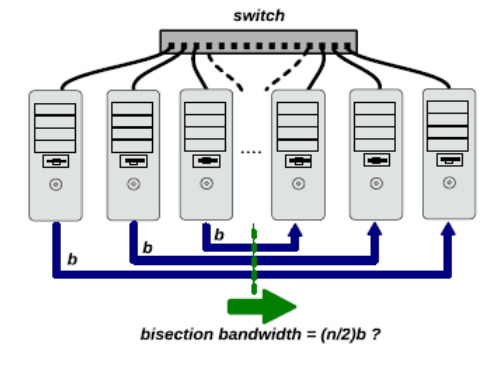
\includegraphics[width=0.40\textwidth]{Images/ej3.png}
\end{figure}

Tomar un número creciente de $n$ procesadores, dividirlos arbitrariamente por la mitad y medir el ancho de banda para esa partición. Comprobar si el ancho de banda de disección crece linealmente con n, es decir si existe algún límite interno para transferencia del switch.

\subsection{Resolución}
\subsubsection{Implementación con MPI}
\lstinputlisting[language=C++]{codigos/main3.cpp}

\subsubsection{Ejecución}
A diferencia de los dos primeros su ejecución se llevó a cabo en uno de los clusters del CIMEC, por lo tanto no se cuenta con ciertos detalles informados en el resto de ejercicios.

\subsubsection{Análisis}
Habiendo finalizado la ejecución obtuve un archivo csv que cargue como DataFrame en python. Como corrí muchas veces el mismo proceso para representar mejor la situación, obtuve el promedio.

Con los datos ya promediados, calculé el ancho de banda de la siguiente forma:

$$b = \frac{\text{Tamaño de paquete}*\text{Nro de procesadores}}{t_{(\text{Nro de procesadores})}}$$

Con estos nuevos cálculos el DataFrame quedó de la siguiente forma: 

\begin{table}[h!]
\centering
 \begin{tabular}{|c |c| c|} 
 \hline
        Nro de procesadores &  Tiempo &  b \\
        \hline
        2.0 &    0.122060 &       5734.875086 \\
        \hline
        4.0 &    0.118834 &       11781.140078 \\
        \hline
        ... &    ... &       ... \\
        \hline
        42.0 &    0.120583 &       121907.428309 \\
        \hline
        44.0 &    0.120362 &        127947.252499 \\
 \hline
 \end{tabular}
 \caption{DataFrame obtenido}
\label{fig:dfej3}
\end{table}

Con estos cálculos ya realizados procedí a graficar tanto el tiempo como el ancho de banda vs. el número de procesadores. (\ref{fig:fig2ej3}, \ref{fig:fig1ej3})

\begin{figure}[H]
    \centering
    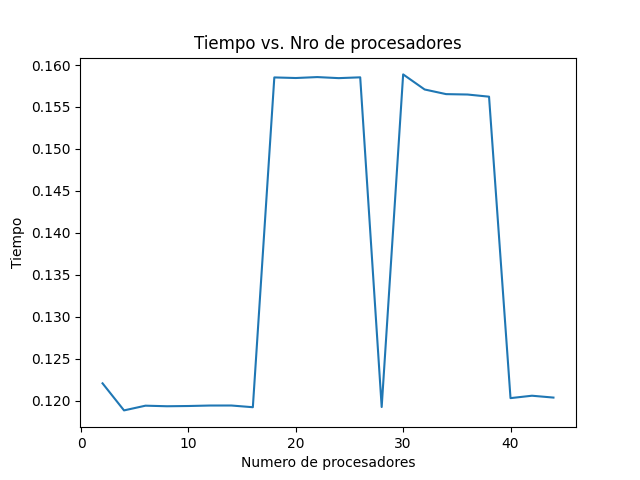
\includegraphics[width=0.60\textwidth]{Images/ej3/fig2ej3.png}
    \caption{Tiempo vs. el número de procesadores}
    \label{fig:fig2ej3}
\end{figure}

\begin{figure}[H]
    \centering
    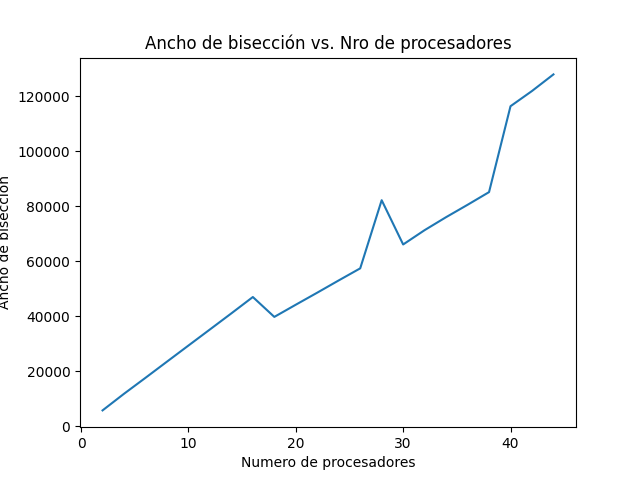
\includegraphics[width=0.60\textwidth]{Images/ej3/fig1ej3.png}
    \caption{Ancho de banda vs. el número de procesadores}
    \label{fig:fig1ej3}
\end{figure}

Como se puede ver observar en la fig \ref{fig:fig2ej3}, el tiempo tiene ciertas irregularidades, pero observando los extremos, podemos ver que no aumenta significativamente. Estas irregularidades pueden deberse a que la configuración de los nodos consta de dos switches distintos. Por otro lado, en la gráfica del ancho de banda no se logra apreciar que se alcance una cota. Este fenómeno se debe a que no se alcanzaron los límites del switch, en caso de disponer de más nodos o enviar un paquete más grande podría alcanzarse. 